\documentclass{beamer}
\usetheme{metropolis}

\usetheme{metropolis}
\usepackage{listings}

\lstdefinestyle{Python}
{
    language=Python,
    basicstyle=\ttfamily\scriptsize,
    keywordstyle=\color{blue}\ttfamily,
	otherkeywords={self,False},
    commentstyle=\color{green!60!black}\ttfamily,
    stringstyle=\color{red!80!black}\ttfamily,
    backgroundcolor=\color{blue!10!white},
    showstringspaces=false,
    numbers=none,
    numberstyle=\tiny,
    numbersep=5pt,
    xleftmargin=2pt,
    framexleftmargin=4pt,
    framexrightmargin=4pt,
    framexbottommargin=5pt,
    framextopmargin=5pt,
    %breaklines=true,
    captionpos=b
}

\lstdefinestyle{MATLAB}{
    language=MATLAB,
    basicstyle=\ttfamily\scriptsize,
    keywordstyle=\color{blue}\ttfamily,
	otherkeywords={classdef,properties,methods},
    stringstyle=\color{red!80!black}\ttfamily,
    commentstyle=\color{green!60!black}\ttfamily,
    numbers=none,
    backgroundcolor=\color{orange!15!white},
    showstringspaces=false,
    numbers=none,
    numberstyle=\tiny,
    numbersep=5pt,
    xleftmargin=2pt,
    framexleftmargin=4pt,
    framexrightmargin=4pt,
    framexbottommargin=5pt,
    framextopmargin=5pt,
    %breaklines=true,
    captionpos=b
}

\lstdefinestyle{output}{
    language=bash,
    basicstyle=\ttfamily\scriptsize,
    keywordstyle=\ttfamily,
    stringstyle=\ttfamily,
    commentstyle=\color{green!60!black}\ttfamily,
    numbers=none,
    backgroundcolor=\color{white},
    showstringspaces=false,
    numbers=none,
    numberstyle=\tiny,
    numbersep=5pt,
    xleftmargin=2pt,
    framexleftmargin=4pt,
    framexrightmargin=4pt,
    framexbottommargin=5pt,
    framextopmargin=5pt,
    %breaklines=true,
    captionpos=b
}

\renewcommand{\emph}[1]{{\color{red}#1}}

\beamerdefaultoverlayspecification{<+->}

\setbeamercolor{block body}{bg=mDarkTeal!30}
\setbeamercolor{block title}{bg=mDarkTeal,fg=black!2}

\title{Test-Driven Development}
\author{Joachim Vandekerckhove}
\date{}


\usepackage{tikz}
\usetikzlibrary{calc,intersections}

\usepackage{amsmath}
\newcommand{\argmin}{\mathop{\mathrm{arg\,min}}}


\usepackage[justification=centering]{caption} % Figures caption

\captionsetup{labelsep = period} 
\usepackage{chngcntr}
\usepackage{ragged2e}
\usepackage[vlined,ruled]{algorithm2e}
\usepackage{comment}
\usepackage{mathtools}
\usepackage{mathrsfs}
\usepackage{wasysym}
\usepackage{marvosym}
\SetKwInOut{Input}{Input}
\SetKwInOut{Output}{Output}


\title{Numerical Optimization}
\author{Joachim Vandekerckhove}
\date{}

\begin{document}

\begin{frame}
  \maketitle
\end{frame}


\begin{frame}{Motivating Problems for Numerical Optimization}

    \begin{itemize}
      \item \textbf{Function Minimization:} Find the minimum of a function $f(x)$ over a given range of $x$.
      \item \textbf{Parameter Estimation:} Given a set of observations, estimate the parameters of a model that best fit the data.
      \item \textbf{Machine Learning:} Train a model to predict outcomes based on input features by minimizing a loss function.
      \item \textbf{Procedure Optimization:} Find the conditions where a certain procedure works best.
    \end{itemize}

\end{frame}


\begin{frame}[fragile]{Numerical optimization in cognitive modeling}
  \begin{itemize}
      \item Cognitive models have parameters that need to be estimated
      \item Estimation means minimizing the \emph{loss $\ell\!\left(x , \theta\right)$}...
      \begin{eqnarray*}
          \hat\theta &=& \underset{\theta}{\mathrm{arg\,min}}
\left(\ell\!\left(x ; \theta\right)\right)
      \end{eqnarray*}
      \item ... or maximizing the \emph{likelihood $f\!\left(x | \theta\right)$}:
      \begin{eqnarray*}
          \hat\theta &=& \underset{\theta}{\mathrm{arg\,max}} \left(f\!\left(x | \theta\right)\right) \\
          &=& \underset{\theta}{\mathrm{arg\,min}} \left(-\log\left(f\!\left(x | \theta\right)\right)\right)
      \end{eqnarray*}
      \item To-be-optimized function is called target or \emph{objective} function
  \end{itemize}
\end{frame}


\begin{frame}[fragile]{Numerical optimization in cognitive modeling}
  Optimization is sometimes possible analytically but most often done using numerical methods:
    \begin{enumerate}
      \item Guess $\theta$ through some method
      \item Compute objective function
      \item Check if the current guess is best yet
      \item Repeat until good enough
    \end{enumerate}
\end{frame}


\begin{frame}[fragile]{Numerical optimization in cognitive modeling}

\begin{algorithm}[H]
  \NoCaptionOfAlgo
  \caption{\textbf{Algorithm:} Abstract Numerical Minimization}
  \Input{objective function $\ell(\theta)$}
  \Output{the learned parameters $\theta$}
  1. Initial guess parameters $\theta$\\
  2. \While{$\ell(\theta)$ is too high}{
    Propose new parameters: $\theta \gets \theta +{} $update;
  }
  3. \textbf{return} $\theta$;
\end{algorithm}

\end{frame}


\begin{frame}[fragile]{Numerical optimization in cognitive modeling}
  \begin{itemize}
     \item Choice of numerical method depends on the problem and available resources, there's \emph{no free lunch}
      \item \emph{Gradient-based optimization} methods use derivatives to search for the minimum
      \begin{itemize}
          \item Derivatives can be approximated using finite differences:
         \begin{enumerate}
           \item Guess $\theta_0$ through some method and compute $\ell(x;\theta_0)$
           \item Guess $\theta_1$ nearby and compute $\ell(x;\theta_1)$
           \item If $\ell(x;\theta_1) < \ell(x;\theta_0)$, move further past $\theta_1$, otherwise move back beyond $\theta_0$
           \item Decrease step size a litte
           \item Repeat until good enough
         \end{enumerate}
      \end{itemize}
      \item Other optimization methods include genetic algorithms, simulated annealing, particle swarm optimization, and the \emph{Nelder-Mead simplex}
  \end{itemize}
\end{frame}


% Gradient Descent:
\begin{frame}{Gradient-based optimization}
    \begin{columns}[T]
        \begin{column}{0.67\textwidth}
        \begin{itemize}
           \item Gradient descent works by iteratively adjusting the model's parameters in the direction of steepest descent of the objective function.\\[1ex]
           \item Newton's method uses the \emph{Hessian matrix} (i.e., the local curvature) to adjust the parameters.\\[1ex]
           \item Quasi-Newton methods approximate the Hessian matrix using a limited amount of information.
        \end{itemize}
        \end{column}
        \begin{column}{0.4\textwidth}
        \begin{figure}
    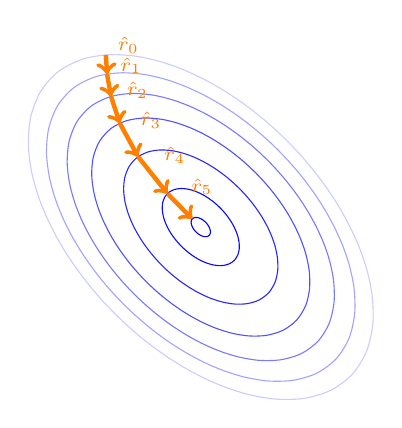
\begin{tikzpicture}[samples=50,smooth,scale=0.6]
            %\clip(-4,-1) rectangle (4,4);
            \path[bend left,name path=arrowcurve] (-2,4) to[out=-30,in=-160] (0,0);
            \foreach \y[count=\i] in {20,16,12,8,4,1,0.0625}{
            \pgfmathsetmacro\colper{\y*4} % color percentage variable
                \draw[name path global/.expanded=curve\i,white!\colper!blue] plot[domain=0:360] ({cos(\x)*sqrt(\y/(sin(2*\x)+2))},{sin(\x)*sqrt(\y/(sin(2*\x)+2))});
                \draw[name intersections = {of ={curve\i} and arrowcurve}](intersection-1) coordinate (P\i);
                \ifnum\i=1 
                    % do nothing
                \else%
                    \pgfmathtruncatemacro\imin{\i-1}
                    \pgfmathtruncatemacro\iprint{\i-2}
                    \draw[->, orange, ultra thick] (P\imin) -- (P\i) node[above right,midway] {\scriptsize $\hat{r}_{\iprint}$}; 
                \fi%
            }     
    \end{tikzpicture}
\end{figure} 
        \end{column}
    \end{columns}
    \vspace{2ex}    
    \begin{itemize}
\item Some nice visualizations: https://www.benfrederickson.com/numerical-optimization/
\end{itemize}
\end{frame}






% Simulated Annealing:

\begin{frame}{Simulated Annealing}
\begin{itemize}
\item Simulated annealing is a powerful \emph{global optimization method} that is inspired by the process of annealing in metallurgy. 
\item  The process is governed by a \emph{temperature} setting that determines the probability of accepting a step in the wrong direction.
\item  A hot algorithm will move randomly, with little regard for the objective function value.  A cold algorithm performs steepest ascent.
\item A slow cooling schedule allows the algorithm to explore many possible peaks before climbing to the top.
\end{itemize}
\end{frame}


\begin{frame}[fragile]{Simulated Annealing}

\begin{algorithm}[H]
\SetAlgoLined
\KwIn{Initial guess $s$, initial temperature $T$; objective $\ell(\theta)$}
\KwOut{Best parameter set found during search}
\While{stopping condition not met}{
Generate new guess $s'$ by random perturbation to $s$;\\
Calculate loss difference $\Delta \ell = \ell(s') - \ell(s)$;\\
\eIf{$\Delta E < 0$}{
Accept $s'$ as the new current state $s$;
}{
Accept $s'$ with probability $\exp(-\Delta \ell/T)$;
}
Decrease temperature $T$;
}
\KwRet{Best state found during search}
\caption{Simulated Annealing Algorithm}
\end{algorithm}

\end{frame}


\begin{frame}[fragile]{Simulated Annealing}
\setlength{\fboxrule}{3pt} 
\framebox{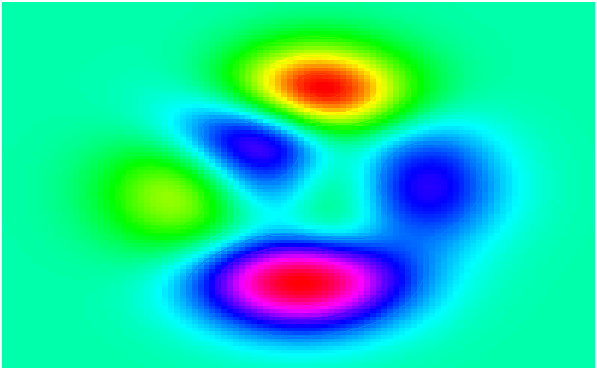
\includegraphics[scale=0.5,bb=10 10 275 165]{anneal-1.png}}
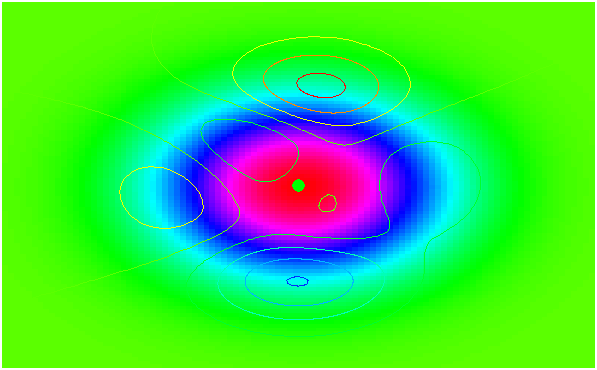
\includegraphics[scale=0.5,bb=0 10 300 190]{anneal0.png}\\
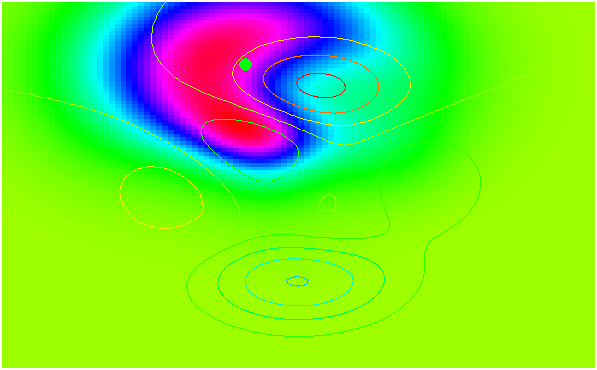
\includegraphics[scale=0.5,bb=0 0 300 190]{anneal1.png}
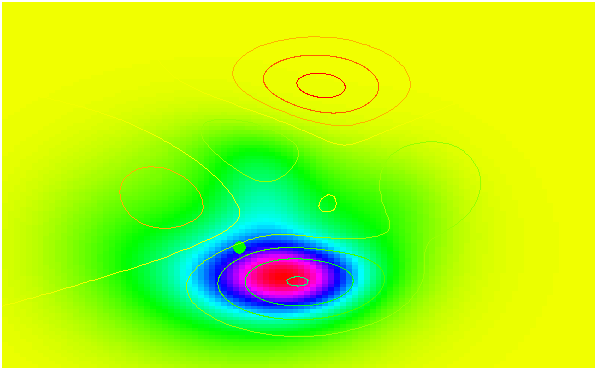
\includegraphics[scale=0.5,bb=10 0 300 190]{anneal2.png}
\end{frame}



\begin{frame}{Constrained vs.\ Unconstrained Optimization}
\begin{itemize}
\item Two main types of optimization problems: constrained and unconstrained
\item In an \emph{unconstrained optimization} problem, the goal is to minimize (or maximize) a function subject to no constraints
\item In a \emph{constrained optimization} problem, the goal is to minimize (or maximize) a function subject to one or more constraints
\item Constrained optimization often requires the use of specialized optimization algorithms and techniques to find the global minimum (or maximum)
\end{itemize}
\end{frame}


\begin{frame}{Constrained vs.\ Unconstrained Optimization}

Constraints can be that some linear transformation $A$ of the parameters must be less than some constant $b$, and/or that some linear transformation $A_{eq}$ of the parameters must be equal to some constant $b_{eq}$, and/or that they must fall in bounds ($l_b$, $u_b$), and/or that some are integers.

\begin{equation*}
\begin{aligned}
& \underset{x}{\text{minimize}}
& & f^\top x \\
& \text{subject to}
& & \begin{Bmatrix}
A x \leq b \text{ (MATLAB) }\\
A x \geq b \text{ (python) }\\
A_{eq} x = b_{eq} \\
l_b \leq x \leq u_b \\
x(\texttt{intflag}) \text{ are integers}
\end{Bmatrix}
\end{aligned}
\end{equation*}

\end{frame}


\begin{frame}
  \frametitle{Unconstrained Example: Production Environment}

\begin{itemize}
\item Imagine a company wants to optimize its production process by finding the optimal temperature and pressure settings for the production equipment.
\item The cost of production is given by:
$$\min_{x} \quad f(x) = e^{(x_1-2)^2 + (x_2-0.5)^2}$$
\item What are the optimal settings to run the production process?
\end{itemize}
\end{frame}


\begin{frame}
  \frametitle{Unconstrained Example: Parameter Estimation}

\begin{itemize}
\item Assume we have some data $D \leftrightarrow \{5, -7, 3, 0, -11\}$
\item We want to describe $D$ with a single number such that the squared distance to each data point is minimal:
$$\min_{x} \quad f(x) = \sum_{i=1}^5 \left(x - d_i\right)^2$$
\item What is the best $x$?
\end{itemize}
\end{frame}


\begin{frame}
  \frametitle{Unconstrained Example: Signal Detection Theory}

\begin{itemize}
\item Assume we have some data $D \leftrightarrow \{$Hits = 4, Misses = 1, False alarms = 2, Correct rejections = 3$\}$
\item Which $(d',c) \leftrightarrow x$ make $D$ most likely:
\begin{eqnarray*}
(\max_{x}) \quad f(x) &=& {5 \choose 4} \theta_H^{5}\left(1-\theta_H\right)^1 \times {5 \choose 2} \theta_F^{2}\left(1-\theta_F\right)^3\\
&&\text{ with }\left\{
\begin{array}{rcl}
\theta_H &=& 1-\Phi\left(-\frac{1}{2}d'+c\right)\\
\theta_F &=& 1-\Phi\left( \frac{1}{2}d'+c\right)
\end{array}\right.\\
\pause
\Rightarrow (\min_{x}) \quad f(x) &=& -\log\left[ \theta_H^{5}\left(1-\theta_H\right)^1 \times  \theta_F^{2}\left(1-\theta_F\right)^3\right]\\
 &=& 
-5\log\left(\theta_H\right)
- \log\left(1-\theta_H\right)\\
&&{\quad}-2\log\left( \theta_F\right)
-3\log\left(1-\theta_F\right)
\end{eqnarray*}
\end{itemize}
\end{frame}


\section{MATLAB}

\begin{frame}[fragile]
\frametitle{Unconstrained Optimization using \texttt{fminsearch}}
$$
\min_{x} \quad f(x) = e^{(x_1-2)^2 + (x_2-0.5)^2}
$$
\begin{itemize}
\item Set up the problem as an anonymous function:
\begin{lstlisting}[style=MATLAB]
% Define the objective function
fcn = @(x) exp( (x(1)-2).^2 + (x(2)-.5).^2);
\end{lstlisting}
\item Minimize using \verb|fminsearch|:
\begin{lstlisting}[style=MATLAB]
% Solve the optimization problem
start = [0, 0];
x = fminsearch(fcn, start);
\end{lstlisting}
\item The solution is $x_1 = 2$ and $x_2 = 0.5$.
\end{itemize}
\end{frame}


\begin{frame}[fragile]{Unconstrained Optimization using \texttt{fminunc}}

        \begin{lstlisting}[style=Matlab]
fcn = @(x) exp( (x(1)-2).^2 + (x(2)-.5).^2);
x0 = [0.5, 1.5];
options = optimoptions('fminunc', 'Display', 'iter', ...
                       'Algorithm', 'quasi-newton', ...
                       'MaxIterations', 1000);
[x, fval, exitflag, output] = fminunc(fcn, x0, options);
        \end{lstlisting}
 
    \begin{itemize}
        \item \texttt{Display=iter} shows optimization progress at each iteration
        \item \texttt{Algorithm} specifies the optimization algorithm to use
        \item \texttt{MaxIterations} sets the maximum number of iterations
        \item Output variables \texttt{x}, \texttt{fval}, \texttt{exitflag}, and \texttt{output} contain the optimization results and information
    \end{itemize}

\end{frame}


\begin{frame}[fragile]{\texttt{fminunc} vs.\ \texttt{fmincon}}

Using \texttt{fminunc}:
        \begin{lstlisting}[style=Matlab]
fcn = @(x)sum((x-[5, -7, 3, 0, -11]).^2);
x0 = 0.5;
[x, fval, exitflag, output] = fminunc(fcn, x0);
        \end{lstlisting}
 
Enforce $x \geq 0$ with \texttt{fmincon}:
        \begin{lstlisting}[style=Matlab]
fcn = @(x)sum((x-[5, -7, 3, 0, -11]).^2);
x0 = 0.5;
[x, fval, exitflag, output] = fmincon(fcn, x0, -1, 0);
        \end{lstlisting}
Note that $A = -1$ and $b=0$, so we enforce that $-x \leq 0$ 

\end{frame}


\begin{frame}[fragile]{MATLAB Optimization Toolbox}

MATLAB has a lot of numerical optimization features.

As of September 2022, the MATLAB Optimization Toolbox User's Guide is 1,584 pages long.  It is an excellent review of modern numerical optimization methods.

\end{frame}


\section{Python}
\addtocounter{framenumber}{-4}
\begin{frame}[fragile]
\frametitle{Unconstrained Optimization using \texttt{scipy.optimize.minimize}}
$$
\min_{x} \quad f(x) = e^{(x_1-2)^2 + (x_2-0.5)^2}
$$
\begin{lstlisting}[style=python]
import numpy as np
import scipy.optimize as optim

# Define the objective function
def fcn(x):
    return np.exp((x[0]-2)**2 + (x[1]-0.5)**2)

# Set the initial point and solve the optimization problem
start = [0, 0]
x = optim.minimize(fcn, start, method='Nelder-Mead')

# The solution is x1=2 and x2=0.5
print(f"The solution is x1={x.x[0]} and x2={x.x[1]}")
\end{lstlisting}

The solution is $x_1 = 2$ and $x_2 = 0.5$.
\end{frame}


\begin{frame}[fragile]{Unconstrained Optimization using \texttt{scipy.optimize.minimize}}

        \begin{lstlisting}[style=python]
import numpy as np
import scipy.optimize as optim

# Define the objective function
def fcn(x):
    return np.exp((x[0]-2)**2 + (x[1]-0.5)**2)

# Set the initial point and solve the optimization problem
x0 = [0.5, 1.5]
options = {'disp': True, 'maxiter': 1000}
x = optim.minimize(fcn, x0, method='BFGS', options=options)
        \end{lstlisting}
 
    \begin{itemize}
        \item \texttt{`disp':True} shows optimization progress at each iteration
        \item \texttt{`maxiter'} sets the maximum number of iterations
        \item \texttt{method=`BFGS'} selects a Quasi-Newton optimization algorithm
    \end{itemize}

\end{frame}


\begin{frame}[fragile]{Unconstrained vs.\ constrained}

        \begin{lstlisting}[style=python]
import numpy as np
import scipy.optimize as optim

# Define the objective function
def fcn(x):
    return np.sum((x - [5, -7, 3, 0, -11])**2)

# Set the initial point
x0 = 0.5
        \end{lstlisting}
 
Unconstrained:
        \begin{lstlisting}[style=python]
x = optim.minimize(fcn, x0)
        \end{lstlisting}
 
Enforce $x \geq 0$ with \texttt{LinearConstraint}:
        \begin{lstlisting}[style=python]
x = minimize(fcn, x0, 
    constraints=optim.LinearConstraint(1, 0))
        \end{lstlisting}
Note that $A = 1$ and $b=0$, so we enforce that $x \geq 0$ 

\end{frame}

\end{document}
